%========================
% main.tex (arXiv-ready)
%========================
\documentclass[10pt,twocolumn]{article}

% ---- Encoding & fonts ----
\usepackage[T1]{fontenc}
\usepackage[utf8]{inputenc}
\usepackage{lmodern}
\usepackage{microtype}           % better typography


% ---- Page geometry & columns ----
\usepackage[a4paper,margin=1in]{geometry}
\setlength{\columnsep}{0.25in}   % space between columns

% ---- Math & symbols ----
\usepackage{mathtools}           % loads amsmath
\usepackage{amssymb,amsthm}
\numberwithin{equation}{section} % equations numbered per section

% ---- Figures & graphics ----
\usepackage{graphicx}
\graphicspath{{figures/}}        % images in ./figures

% ---- Tables ----
\usepackage{booktabs}            % nice rules
\usepackage{array}
\usepackage{makecell}            % header wrapping / multi-line cells
\usepackage[table]{xcolor}       % table shading
\usepackage{siunitx}
\sisetup{detect-all}

% ---- Captions & subfigures (order matters: caption BEFORE subcaption) ----
\usepackage[labelfont=bf]{caption}
\usepackage{subcaption}

% ---- Floats ----
\usepackage{stfloats}            % allow bottom placement of double-column floats
\usepackage{placeins}            % \FloatBarrier
\setlength{\dbltextfloatsep}{8pt plus 2pt minus 2pt} % space between dbl-floats and text
\renewcommand{\textfraction}{.05}
\renewcommand{\dbltopfraction}{.95}
\renewcommand{\dblfloatpagefraction}{.9} % avoid float-only pages

% ---- Links & bibliography ----
\usepackage[numbers,sort&compress]{natbib}
\usepackage[hidelinks]{hyperref} % load hyperref near-last

% ---- Misc helpers ----
\usepackage{xifthen}             % for conditional figure placeholders
\usepackage[normalem]{ulem}      % \uline etc., keep \emph behavior
\usepackage{supertabular}        % multipage tables in twocolumn

% ---- Macros ----
\newcommand{\Stirling}[2]{\genfrac\{\}{0pt}{}{#1}{#2}}
% Accidentals in running text
\newcommand{\nflat}{\ensuremath{\flat}}
\newcommand{\nsharp}{\ensuremath{\sharp}}
\newcommand{\nnatural}{\ensuremath{\natural}}

\date{\today}

% --- Title/authors ---
\title{Uniqueness on a Continuum: Quantifying Tonal Ambiguity Using Information Theory}
\author{Michael Seltenreich$^{1}$\\[4pt]
\small $^{1}$Anthropic PBC\\
\small \texttt{michaelsel@anthropic.com}
}

\begin{document}
    \twocolumn[
        \maketitle
        % NOTE: Material in this optional argument is typeset full-width automatically.
        \begin{abstract}
            We propose a continuous measure of tonal ambiguity that builds on the established concept of uniqueness.
            While uniqueness is widely regarded as necessary for tonality, it cannot (i) discriminate among sets that possess it, (ii) capture hierarchical organization in modes of limited transposition, or (iii) account for temporal unfolding
            To address these limitations, we introduce a companion measure that quantifies the degree of tonal ambiguity in a set, grounded in information theory.
            The measure applies across pitch‑class sets and tuning systems, yielding a continuous assessment of tonal ambiguity.
            It expands analytic coverage of tonal relationships and offers a practical tool for theory and analysis.
        \end{abstract}
        \vspace{2em}
    ]

    \section{Introduction}\label{sec:intro}

    Tonality lies at the base of many of the world's musical cultures and is fundamental to Arabic and Turkish maqamat \citep{Farraj2019,Signell2008}, Hindustani and Carnatic ragas \citep{Castellano1984}, and much of Western music \citep{KrumhanslKeil1982}.
    It can be defined as the hierarchical organization of a scale's notes into distinct functional roles, with one note typically serving as the central “tonic” (arrival point) and another as a contrasting “dominant” (recitation) tone.
    \citet{Balzano1982} argues that, as a prerequisite for such hierarchy to emerge among a set’s members, the set must possess a structural property called “uniqueness.”
    This claim was recently supported by \citet{Pelofi2021}, who showed empirically that melodic statistical dependencies are learned more effectively in sets that exhibit uniqueness.

    A scale exhibits \textit{uniqueness} when relations among its notes permit a single unambiguous transposition.
    This property enables listeners to orient themselves within the conceptual space defined by the scale’s internal relationships.
    \autoref{fig:shapes}A illustrates this with two pentagons: the left demonstrates uniqueness; the right does not.
    The distinction lies in the edges: those on the left occur in two different sizes (yellow and orange), whereas those on the right are uniform.
    As shown in \autoref{fig:shapes}B, after an unknown rotation the unique pentagon can be reoriented to its original position with certainty.
    In contrast, the uniform pentagon cannot be uniquely restored, as its five identical edges yield multiple indistinguishable rotations.

    \begin{figure}[htbp]
        \centering
        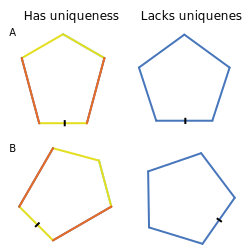
\includegraphics[width=\linewidth]{figures/two-shapes}%
        \caption{A) Two pentagons differing in structural properties: the left, with sides of two distinct lengths (yellow and orange), exhibits uniqueness; the right, with five equal sides, lacks uniqueness.
        B) After rotation, only the unique pentagon can be reoriented unambiguously, whereas the uniform pentagon admits multiple indistinguishable orientations.}
        \label{fig:shapes}
    \end{figure}

    The same structural idea carries over to musical scales.
    For example, the major scale exhibits uniqueness, allowing us to identify C–D–E–F–G–A–B unambiguously as the key of C (or one of its modes) rather than as any of its 11 other transpositions; its internal structure makes the orientation clear.
    By contrast, scales that lack uniqueness resist such identification.
    Consider the whole‑tone scale: C–D–E–F$\sharp$–G$\sharp$–B$\flat$ cannot be definitively labeled as a “C whole‑tone scale” or a “D whole‑tone scale,” since its uniform structure renders every pitch an equally plausible tonic.
    Consequently, the label “C whole‑tone scale,” which implies a privileged tonic, is misleading.
    In this respect, the whole‑tone scale parallels the uniform pentagon in \autoref{fig:shapes}, as both structures lack uniqueness.
    \citet{Balzano1982} argues that uniqueness is necessary for the emergence of tonality, since the assignment of hierarchical roles depends on unambiguous relations among a scale’s notes.
    Formally this may be true, yet in practice listeners likely tolerate some tonal ambiguity.
    Thus, a binary framing may obscure more graded tonal interpretations in scales that lack strict uniqueness.
    Notably, the modes of limited transposition—among them the whole‑tone scale—have long attracted composers precisely because they resist a single unambiguous transposition.
    Nonetheless, these modes are more structured than atonality: they admit strictly more than one tonal interpretation, but strictly fewer than twelve \citep{Messiaen1944}.
    This position allows them to support both chromaticism and modulation, albeit within clear structural constraints.

    Uniqueness splits scales into two classes—those that have it and those that do not—but it offers little guidance about \emph{how strongly} a set points to a tonic.
    Modes of limited transposition, for instance, lack a clear tonality yet still manifest a degree of hierarchical structure.
    At the most fundamental level, this hierarchy distinguishes between notes that belong to the scale and those that do not (chromatic notes).
    For such scales, uniqueness is by definition absent and thus becomes irrelevant.
    Nevertheless, they project a distinct musical identity that arbitrary note collections do not.
    This suggests the need for a more nuanced, continuous measure to capture the extent to which hierarchical relationships can emerge even without uniqueness.

    Likewise, the uniqueness property gives only a blunt perspective on scales that \emph{do} possess it.
    Even among unique scales, some structures yield a far more salient sense of transposition than others.
    Moreover, uniqueness concerns a scale as a whole, yet music unfolds sequentially; thus uniqueness may not be immediately apparent even in scales that formally possess it.

    For instance, although the major scale possesses uniqueness, the tonal center of \emph{Twinkle, Twinkle, Little Star} cannot be determined unambiguously at the outset.
    The first measure (C–G–A–G) is compatible with as many as six major keys (see candidate tonics under the passage in \autoref{fig:twinkle}).
    As the melody unfolds, A$\natural$ rules out both E$\flat$ and A$\flat$ major; F$\natural$ excludes G major; and later E$\natural$ eliminates B$\flat$ major.
    Ultimately, the melody narrows to interpretations in either C or F major, since the absence of a decisive B$\natural$ or B$\flat$ leaves the final tonic (formally) ambiguous.

    Of course, listeners determine a passage’s tonic using many features beyond a tally of pitches.
    For a thorough treatment, see \citet{LerdahlJackendoff1983} and related work \citep{BharuchaKrumhansl1983,Lerdahl2004,Patel1998,Thompson1997}.
    The preceding example simply illustrates the point; it does not suggest that the tonic of \emph{Twinkle, Twinkle, Little Star} is unknowable.
    In practice, listeners often infer underlying scale constituents even when they are not explicitly stated.
    Nonetheless, the passage underscores that uniqueness need not be explicitly expressed for a coherent tonal hierarchy to emerge.

    Importantly, passages like this resemble those belonging to modes of limited transposition in that neither succeeds in structurally identifying a tonic—at least not initially or explicitly—yet both narrow the universe of candidate tonics from twelve to a small subset.

    \begin{figure*}[htbp]
        \centering
        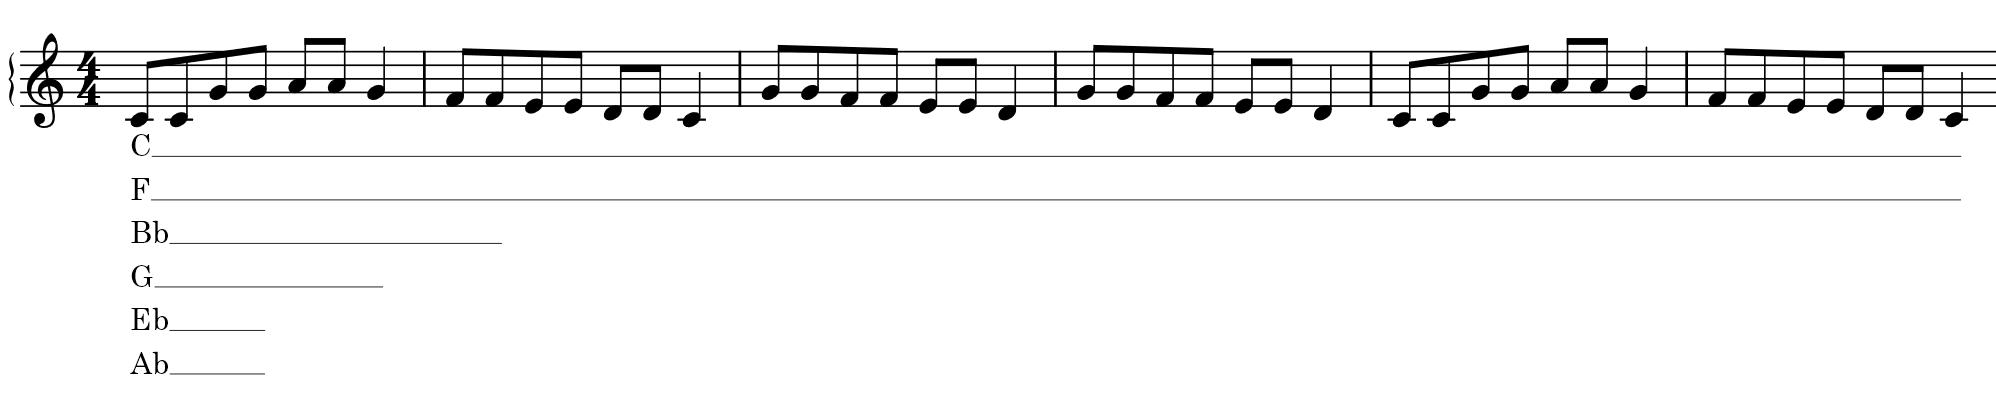
\includegraphics[width=0.9\textwidth]{figures/twinkle}%
        \caption{\emph{Twinkle, Twinkle, Little Star} with possible tonal interpretations marked below.}
        \label{fig:twinkle}
    \end{figure*}

    In Western practice, tonal ambiguity often lies at the base of musical expression and underpins an important aspect of the art form \citep{NodenSkinner1984, Richards2017, Smith1992, Temperley2007, Uchida1990}.
    To make the challenge concrete, consider the widely prevalent anhemitonic pentatonic set (02479).
    It transparently illustrates how our ability to determine a scale’s transposition is context‑dependent.
    In this set, the appearance of any single note shrinks the space of possible transpositions to one of five possibilities—any given note may serve as one of five scale degrees and, correspondingly, as the tonic of each of five candidate tonics.
    \autoref{fig:necklaces}A illustrates this reduction: when a single pitch is specified (white node), only five transpositions of the set remain (shown in set‑theoretical notation and as pentagons; see caption for details).

    \begin{figure*}[htbp]
        \centering
        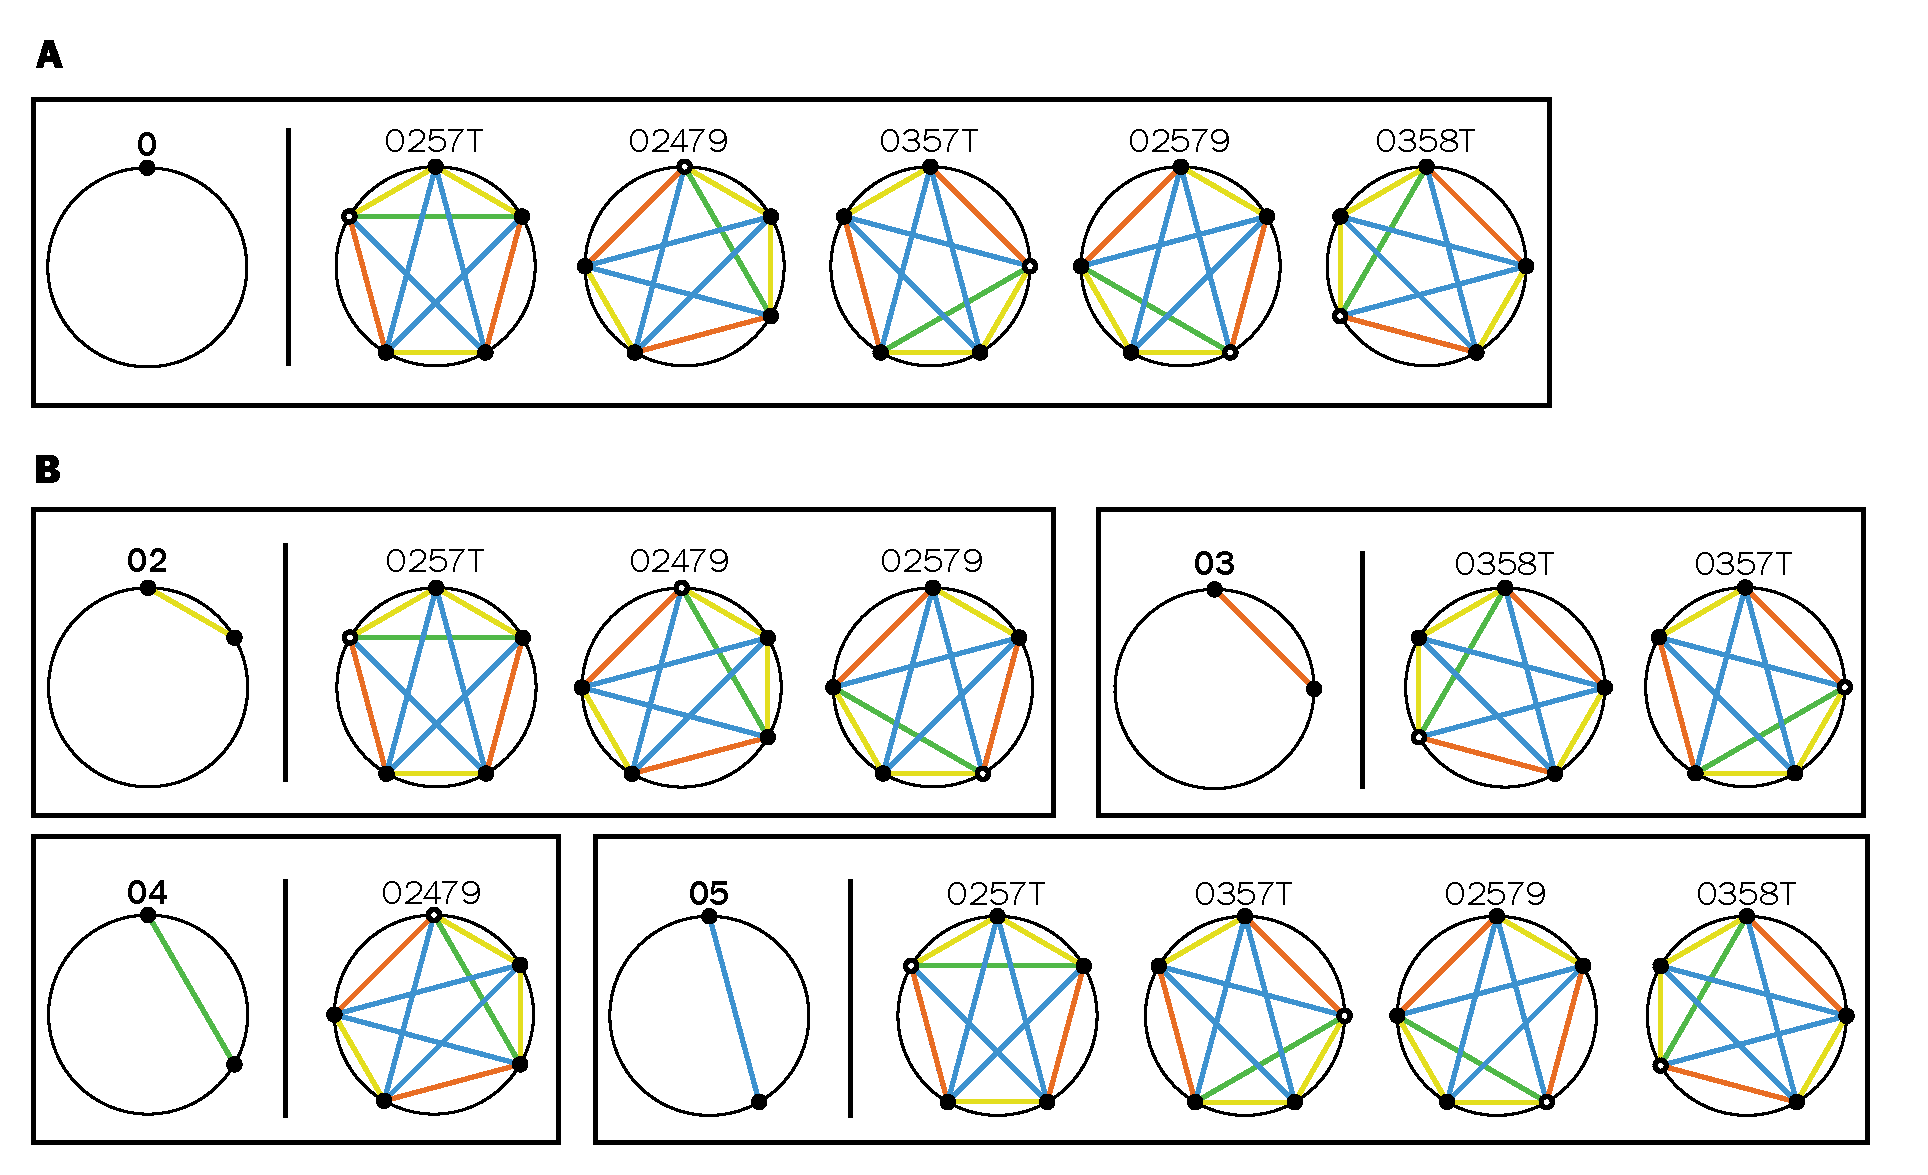
\includegraphics[width=0.9\textwidth]{pentatonic-necklaces}%
        \caption{The anhemitonic pentatonic scale (02479) represented as a pentagon, with edge lengths proportional to composite interval sizes (yellow = 2 semitones, orange = 3, green = 4, blue = 5).
        A white circle marks pitch‑class 0 (prime‑form orientation).
        \textbf{A)} The five transpositions of 02479 containing pitch‑class 0.
        \textbf{B)} Remaining candidate transpositions given intervals 02, 03, 04, and 05, respectively.}
        \label{fig:necklaces}
    \end{figure*}

    While one note always leaves five possibilities, the informational value of a second pitch depends on the set’s structure and the identity of that pitch.
    As shown in \autoref{fig:necklaces}B, the second note may provide very different amounts of information.
    In some cases (e.g., 04), the specific transposition is determined unambiguously—C and E occur only in \textbf{\uline{C}}–D–\textbf{\uline{E}}–G–A.
    Other intervals (e.g., 05) may leave as many as four of the five candidates; for C and F, the set can be
    B$\flat$–\textbf{\underline{C}}–D–\textbf{\underline{F}}–G,\quad
    E$\flat$–\textbf{\underline{F}}–G–B$\flat$–\textbf{\underline{C}},\quad
    \textbf{\underline{F}}–G–A–\textbf{\underline{C}}–D,\quad
    A$\flat$–B$\flat$–\textbf{\underline{C}}–E$\flat$–\textbf{\underline{F}}.

    These observations suggest that, to capture tonal potential not only in modes of limited transposition but also in scales that formally possess uniqueness, we require a measure that goes beyond a binary classification.
    Such a measure must reflect that music unfolds sequentially and that tonal clarity often emerges gradually.
    To this end, I introduce a metric analogous to uniqueness but defined continuously, expressing degrees of tonal ambiguity (or certainty).
    Methods from information Theory provide a rigorous framework for such a measure, allowing us to calculate precisely how much tonal uncertainty remains given an arbitrary collection of pitches.

    The remainder of this paper is organized as follows.
    Section~\ref{sec:core} presents the core concepts and practical applications of the proposed measure.
    Section~\ref{sec:math-dev} then gives a complete mathematical development with pedagogical exposition, beginning with an accessible introduction to information theory and proceeding to derive the measure and explore its implications across various musical scales.


    \section{Core Concepts and Applications}\label{sec:core}

    \noindent\textbf{Who this section is for.}
    Readers who want the \emph{bottom line}: what the paper introduces, how to compute it, and how to use it—without the full pedagogical build‑up in \S\ref{sec:math-dev}.

    \subsection*{What this paper contributes}
    \begin{enumerate}
        \item A \emph{continuous} measure of tonal ambiguity for any pitch‑class collection $S$ in any EDO, extending the binary notion of \emph{uniqueness}.
        \item A principled aggregation of information across subset sizes (dyads, trichords, \dots, up to $|S|$) into a single set‑level quantity.
        \item A time‑aware variant that models melodies as draws \emph{with repetition} and weights results by the expected number of \emph{distinct} pitches.
        \item A cross‑set ``disambiguation'' view: how observed notes rule in/out \emph{which} common scale family is likely, not only \emph{which transposition}.
    \end{enumerate}

    \subsection*{Key quantities (use these; derivations in \S\ref{sec:math-dev})}
    Let $c$ be the size of the chromatic space (e.g., $c=12$ in 12‑EDO), and let $S\subset\mathbb{Z}_c$ be a pitch‑class set of size $m=|S|$. For an observed combination $X\subset\mathbb{Z}_c$ of $k$ distinct pitch classes:
    \begin{itemize}
        \item \textbf{Remaining tonal interpretations within $S$.}
        \[
            t_S(X) \coloneqq \bigl|\{\tau\in \mathbb{Z}_c : X \subseteq \tau{+}S\}\bigr|.
        \]
        This is the number of \emph{candidate tonics} that remain possible for $S$ given $X$. For modes of limited transposition, $t_S(X)$ naturally reflects rotational symmetries.

        \item \textbf{Self‑information provided by $X$ (bits).}
        \[
            I_S(X) \coloneqq \log_2\!\left(\frac{c}{t_S(X)}\right).
        \]
        We measure information in bits (base‑2 logs); smaller $t_S(X)$ means more information.

        \item \textbf{Cardinality‑$k$ expected information (bits).}
        \[
            \mathbb{E}_{\Omega_k(S)}[I]
            \coloneqq \frac{1}{\binom{m}{k}} \sum_{\substack{X\subseteq S\\ |X|=k}} I_S(X).
        \]
        Grouping isomorphic combinations (e.g., by interval class for dyads) yields the same value with combinatorial weights; for dyads these weights are the entries of the interval vector.

        \item \textbf{Set‑level measure and its musical reading.}
        Averaging over all non‑empty cardinalities,
        \[
            \mathbb{E}_S[I]
            \coloneqq \sum_{k=1}^{m}\!\left(\frac{\binom{m}{k}}{2^m-1}\right)\,\mathbb{E}_{\Omega_k(S)}[I].
        \]
        Report the \emph{average number of tonal interpretations}
        \[
            \boxed{\;\bar{t}(S)=\dfrac{c}{2^{\mathbb{E}_S[I]}}\;}
        \]
        We refer to $\bar{t}(S)$ as the \emph{Tonal Ambiguity Index} (TAI).
    \end{itemize}

    \paragraph{Time‑aware variant (melodic draws).}
    If a passage contains $n$ notes drawn with repetition from $S$ of size $m$, let $P_k$ be the probability that these $n$ draws yield exactly $k$ \emph{distinct} pitch classes:
    \[
        P_k \;=\; m^{-n}\,\Stirling{n}{k}\,\binom{m}{k}\,k!
        \qquad\text{(Eq.~\ref{eq:Pk}).}
    \]
    Then the expected information and its musical reading for an $n$‑note passage are
    \[
        \mathbb{E}_S[I \mid n] \;=\; \sum_{k=1}^{m} P_k \,\mathbb{E}_{\Omega_k(S)}[I],
        \qquad
        \bar{t}_n(S) \;=\; \frac{c}{2^{\mathbb{E}_S[I \mid n]}}.
    \]
    In practice, $n{=}8$ offers a good balance: long enough to distinguish 8‑note sets (e.g., octatonic) yet short enough to avoid trivial convergence.

    \subsection*{How to compute it (minimal recipe)}
    \begin{enumerate}
        \item \textbf{Fix the universe.} Choose $c$ (e.g., $12$) and a set $S$ (e.g., major, pentatonic, octatonic).
        \item \textbf{Precompute coverage.} For each $\tau\in \mathbb{Z}_c$, form $\tau{+}S$ and record which $X$ (at each $k$) occur.
        \item \textbf{For each $k$.} For all $X{\subseteq}S$ with $|X|{=}k$, compute $t_S(X)$ and $I_S(X)=\log_2(c/t_S(X))$; average to get $\mathbb{E}_{\Omega_k(S)}[I]$.
        \item \textbf{Aggregate.} Combine across cardinalities with the binomial weights to get $\mathbb{E}_S[I]$ and report $\bar{t}(S)=c/2^{\mathbb{E}_S[I]}$.
        \item \textbf{Optional: time‑aware.} Weight by $P_k$ to obtain $\bar{t}_n(S)$.
    \end{enumerate}

    \subsection*{Diagnostic combinations and cross‑set use}
    \begin{itemize}
        \item \textbf{Diagnostic within a set.} $X$ is \emph{diagnostic} for $S$ if $t_S(X)=1$ (it pins down the tonic/transposition). In the diatonic set, several trichords containing IC\,6 are diagnostic (Table~\ref{tab:trichords}, Fig.~\ref{fig:cadential}).
        \item \textbf{Disambiguating between scale families.} For a family $\mathcal{F}$ (e.g., \{major, harmonic minor, melodic minor, pentatonic, whole‑tone, octatonic\}), define
        \[
            t_{\mathcal{F}}(X) \;=\; \bigl|\{\,S\in\mathcal{F}:\exists\,\tau \text{ s.t. } X\subseteq \tau{+}S\,\}\bigr|.
        \]
        The disambiguation gain is $D_{\mathcal{F}}(X)=\log_2(|\mathcal{F}|/t_{\mathcal{F}}(X))$ (bits): how many families survive after hearing $X$.
    \end{itemize}

    \subsection*{Headline results (at a glance)}
    Values are $\bar{t}(S)$, the average number of viable tonal interpretations (smaller = less ambiguous).
    \begin{itemize}
        \item \textbf{Common sets with uniqueness.} Major $\approx 2.42$; Pentatonic $\approx 2.29$; Melodic minor $\approx 1.92$; Harmonic minor $\approx 1.87$ (Table~\ref{tab:tonal-interpretations}).
        \item \textbf{Modes of limited transposition.} Whole‑tone $\approx 6.00$ (flat across $k$); Octatonic $\approx 4.33$; Augmented $\approx 3.49$ (Table~\ref{tab:tonal-interpretations-mlt}).
        \item \textbf{Temporal convergence (8‑note draws).} Major, harmonic minor, and ascending melodic minor approach uniqueness quickly ($\bar{t}_8(S)\!\approx\!1$); pentatonic converges more slowly; whole‑tone remains at $6$; octatonic approaches $\sim 4$ (Fig.~\ref{fig:wide}).
    \end{itemize}

    \subsection*{Practical ways to use the metric}
    \begin{enumerate}
        \item \textbf{Analysis.} Given notes $X$ heard in context $S$, report $t_S(X)$ and $I_S(X)$ in bits. Example (diatonic): dyad 01 leaves $t{=}2$ ($\approx 2.58$ bits), while 05 often leaves $t{=}6$ ($1$ bit).
        \item \textbf{Comparing scales.} Prefer smaller $\bar{t}(S)$ for faster \emph{tonal induction}; prefer larger $\bar{t}(S)$ to \emph{sustain} ambiguity.
        \item \textbf{Compositional design.} Use diagnostic combinations ($t{=}1$) to engineer cadential clarity; avoid them (or use high‑$t$ combinations) to prolong ambiguity.
        \item \textbf{Pedagogy / cognition.} $\bar{t}_n(S)$ predicts how quickly different sets yield stable tonic inferences as note evidence accrues.
    \end{enumerate}

    \subsection*{Assumptions, knobs, and extensions (brief)}
    \begin{itemize}
        \item The default assumes all $k$‑subsets of $S$ are equally likely; style‑specific weights (e.g., corpus‑derived) can replace the uniform model in $\mathbb{E}_{\Omega_k(S)}[I]$.
        \item Replace $c{=}12$ with any EDO (or any finite chromatic universe) to extend beyond 12‑EDO.
        \item The present metric is pitch‑class based; timbre, meter, voice‑leading, and duration are orthogonal cues you may layer on in other models.
    \end{itemize}



    \section{Mathematical Development}\label{sec:math-dev}

    \textit{The following sections provide detailed derivations and pedagogical exposition of the concepts introduced above.
Readers seeking to understand the mathematical foundations or looking for a gentler introduction to information theory in musical contexts should continue here.}


    \subsection{A "bit" about information Theory}

    As argued above, the dichotomous framing of uniqueness fails to capture the gradient nature of tonal ambiguity, highlighting the need for a more continuous metric.
    Information Theory, a subdiscipline of data science concerned with the quantification of information \citep{shannon1948}, offers a promising framework for such a measure.
    At its core, the principle is simple: the rarer an event, the more information it provides.

    A familiar analogy is the word‑guessing game hangman, where the goal is to identify a hidden word by guessing letters one at a time.
    Correctly guessing a rare letter such as "Z" reduces the pool of candidate words more than guessing a common letter such as "A," since fewer words contain "Z."
    As more letters are revealed, the set of possibilities shrinks until only a single word remains.

    The same logic applies to tonality.
    Here, instead of uncovering a hidden word, we seek to identify the tonic of a passage; and instead of adding letters, we add notes.
    Suppose we listen in the context of the major scale.
    Hearing the note F immediately reduces the candidate tonalities from twelve to the seven major keys that contain F (F, G$\flat$, A$\flat$, B$\flat$, C, D$\flat$, and E$\flat$).
    In doing so, it excludes G, A, B, D, and E major.
    Adding a second pitch narrows the field further: for instance, the co‑occurrence of F and E restricts the possibilities to just two scales—C major and F major—since these are the only major keys containing both notes.

    This process can be formalized using the concept of \textit{self}\textit{‑}\textit{information}, which measures the information gained from a given event.
    It is defined as:

    \begin{align}
        I(E) &= \log_{2} \left( \frac{1}{p(E)} \right), \\
        E &:\ \text{some event}, \\
        p(E) &:\ \text{the probability of this event to occur}.
    \end{align}


    Although the formula may appear abstract, its meaning is intuitive.
    The unit of measure here is the \textit{bit}, representing the amount of information needed to halve the remaining possibilities.
    For example, if there are initially 100 possible outcomes, one bit of information reduces the pool to 50; two bits reduce it further to 25.

    In Western tonal music, the initial space of possibilities typically consists of the twelve major or minor tonics.
    Acquiring 1 bit of information cuts this space from 12 to 6; 2 bits reduce it to 3.
    To determine the key unambiguously, the space must shrink from 12 to 1, which requires approximately 3.585 bits.
    Put differently, identifying the tonic in Western music entails resolving an initial uncertainty of 3.585 bits.

    \subsection{The Diatonic Set}

    When a note is randomly selected from the diatonic set, the number of possible transpositions decreases from 12 to 7, since that note may serve as any of the scale's degrees.
    This mirrors the case of the pentatonic set, where a single note reduces the transpositional space from 12 to 5.
    As with the pentatonic scale (see \autoref{fig:necklaces}B), however, the impact of adding a second note depends heavily on which note is chosen.
    Previously, we illustrated this variability through exhaustive listing, but as the size of the set increases, such enumeration quickly becomes impractical—especially when considering combinations beyond pairs of notes.
    To address this more effectively, we turn to information Theory, which allows us to quantify the information contributed by each combination.

    In the diatonic set, two‑note combinations vary widely in the information they provide.
    \paragraph{Example.}
    In 12‑EDO ($c=12$), the dyad 05 (C–F) leaves six candidate tonics
    $\{C,D\flat,E\flat,F,A\flat,B\flat\}$, so $t_S(X)=6$ and $I_S(X)=\log_2(12/6)=1$ bit.
    By contrast, the dyad 01 leaves $t_S(X)=2$ (e.g., $D\flat$ or $A\flat$ if $0{=}$C), i.e., $\approx 2.58$ bits.

    Formally, the information gained from a given note combination can be calculated as:
    \begin{equation}
        I_S(X) \;=\; \log_{2}\!\left(\frac{c}{t_S(X)}\right).
        \label{eq:derivingSelfInformation}
    \end{equation}
    \footnote{Sketch: Let $T\in\mathbb{Z}_c$ be the (unknown) tonic with a uniform prior. Given a combination $X$, the surviving tonics form a set of size $t_S(X)$ and $T\mid X$ is uniform on it; hence $H(T)=\log_2 c$, $H(T\mid X)=\log_2 t_S(X)$, and the information gain is $I=H(T)-H(T\mid X)=\log_2(c/t_S(X))$. For non‑uniform priors, replace $c$ and $t_S(X)$ by $2^{H(T)}$ and $2^{H(T\mid X)}$.}
    We measure information in bits (base‑2 logarithms). Put simply, $c$ is the size of the chromatic space (12 in 12‑EDO) and $t_S(X)$ is the number of candidate \emph{tonics} (i.e., tonic pitch classes) that remain possible given $X$.

    Thus, 01 yields approximately $2.58$ bits, while 05 yields $1$ bit. Conversely, the number of remaining tonics can be recovered from bits of information as
    \begin{equation}
        t_S(X) \;=\; \frac{c}{2^{\,I_S(X)}}.
        \label{eq:remaining_transpositions}
    \end{equation}

    Table~\ref{tab:diatonic-2note} summarizes the information values for all two‑note combinations in the diatonic set, showing both the number of candidate tonics and their associated probabilities based on the interval vector $\langle 2,5,4,3,6,1\rangle$.

    \begin{table}[htbp]
\centering
\caption{Information-theoretic values for 2-note combinations in the diatonic set.
Columns list: pitch class combination, number of candidate transpositions ($t$),
information in bits ($I(E)$), number of instances in the scale, and the probability
of each combination occurring $p(x)$.}
\label{tab:diatonic-2note}
    \begin{tabular}{l c c c c}
    \toprule
    \makecell[l]{Pitch Class\\Combination} & $t$ & $I(E)$ &
    \makecell[c]{Instances\\in scale} & $p(x)$ \\
    \midrule
    01 & 2 & 2.58 & 2 & 2/21 \\
    02 & 5 & 1.26 & 5 & 5/21 \\
    03 & 4 & 1.58 & 4 & 4/21 \\
    04 & 3 & 2.00 & 3 & 3/21 \\
    05 & 6 & 1.00 & 6 & 6/21 \\
    06 & 2 & 2.58 & 1 & 1/21 \\
    \bottomrule
    \end{tabular}
\end{table}

    We refer to the number of candidate \emph{tonics}—i.e., pitch classes that can serve as the tonic under set $S$ given the observed notes—as the extent of tonal ambiguity.
    However, it is important to recall that uniqueness is a property of the set as a whole, not of specific subsets.
    Thus, while computing tonal ambiguity for particular note combinations is useful, it does not by itself capture the overall tonal clarity captured by the set.
    To do so, we must weigh the high information gained from rare combinations against their low probability of occurring.

    The earlier hangman analogy makes this clear.
    Correctly guessing the letter "Z" provides more information than guessing "A," but "Z" is also much less likely to be correct in the first place.
    Similarly, in a musical context, highly diagnostic note combinations (such as rare intervals) may drastically narrow the set of possibilities, but their infrequent occurrence means they contribute less to the average experience of tonal induction.
    Thus, we need a method that balances the information each combination provides with the likelihood of its appearance.

    For this, we turn to the average information (often termed “entropy” in this paper for brevity), following \citet{shannon1948}.
    Formally:

    \begin{equation}
        \mathbb{E}[I] = \sum_{x} p(x) \cdot I[E]
        \label{eq:expected-info}
    \end{equation}

    Where $p(x)$ is the probability of a certain interval-class (or note-combination) $x$ occurring in the (diatonic or other) set, and $I[E]$ is the self-information of that note-combination.
    Applying this to the diatonic set yields:

    \begin{align}
        \mathbb{E}_{\text{set}~\Omega_{2}}[I] \;\approx\; &
        \underbrace{\left( \frac{2}{21} \cdot 2.58 \right)}_{\substack{\text{01:}\\ p(x)\cdot I(E)}} +
        \left( \frac{5}{21} \cdot 1.26 \right) +
        \left( \frac{4}{21} \cdot 1.58 \right)
        \notag \\[4pt]
        &+ \left( \frac{3}{21} \cdot 2.00 \right) +
        \left( \frac{6}{21} \cdot 1.00 \right)
        \notag \\[4pt]
        &+ \left( \frac{1}{21} \cdot 2.58 \right)
        \;\approx\; 1.55
        \label{eq:expectation-example}
    \end{align}

    This result indicates that, on average, a two‑note combination reduces the space of possible transpositions by a factor of $2^{1.55} \approx 2.93$, leaving about $4$ viable options out of $12$.

    Interestingly, the comparison between the number of instances of each interval and the number of candidate transpositions reveals a striking pattern.
    In most cases, these values coincide; the exception is IC6, which occurs once (e.g., 5–11) but still allows two candidate transpositions (C major or G$\flat$ major if 0 = C).
    This discrepancy reflects the special case of symmetrical divisions of the octave (e.g., 06, 048, 0369, 02468T), which yield rotational symmetries and underpin modes of limited transposition.
    Thus, entropy effectively captures the tonal ambiguity arising from such symmetries.

    While this entropy measure provides a richer view than raw two-note statistics, it remains limited to pairs.
    To better understand tonal ambiguity, we extend the analysis to trichords.
    The same method applies: we calculate the self-information of each trichord, weighted by its probability of occurrence within the set.
    Unlike dyads, however, probabilities cannot be derived directly from the interval vector.
    Instead, we enumerate the trichords present in the set, using the binomial coefficient formula $\binom{n}{k} = \frac{n!}{(n-k)! \, k!}$ to determine the total number of trichords (35 in a 7‑note set).

    \begin{table}[htbp]
    \centering
    \caption{Information values for all trichords in the diatonic set.
    Columns list: combination, information in bits ($I(E)$), probability of occurrence $p(x)$,
    and number of instances in the set.}
    \label{tab:trichords}
    \begin{tabular}{l c c c}
        \toprule
            \makecell[c]{Combination} &
            \makecell[c]{$I(E)$} &
            \makecell[c]{$p(x)$} &
            \makecell[c]{Instances\\in the set} \\
        \midrule
            012 & 0.00 & 0.000 (0/35) & 0 \\
            013 & 2.58 & 0.057 (2/35) & 2 \\
            014 & 0.00 & 0.000 (0/35) & 0 \\
            015 & 2.58 & 0.057 (2/35) & 2 \\
            016 & 3.58 & 0.029 (1/35) & 1 \\
            023 & 2.58 & 0.057 (2/35) & 2 \\
            024 & 2.00 & 0.086 (3/35) & 3 \\
            025 & 1.58 & 0.114 (4/35) & 4 \\
            026 & 3.58 & 0.029 (1/35) & 1 \\
            027 & 1.26 & 0.143 (5/35) & 5 \\
            034 & 0.00 & 0.000 (0/35) & 0 \\
            035 & 1.58 & 0.114 (4/35) & 4 \\
            036 & 3.58 & 0.029 (1/35) & 1 \\
            037 & 2.00 & 0.086 (3/35) & 3 \\
            045 & 2.58 & 0.057 (2/35) & 2 \\
            046 & 3.58 & 0.029 (1/35) & 1 \\
            047 & 2.00 & 0.086 (3/35) & 3 \\
            048 & 0.00 & 0.000 (0/35) & 0 \\
            056 & 3.58 & 0.029 (1/35) & 1 \\
        \bottomrule
    \end{tabular}
\end{table}

    As Table~\ref{tab:trichords} shows, certain trichords alone are sufficient to uniquely identify the scale's transposition.
    We term these \textit{diagnostic combinations}, as they effectively diagnose the set's identity from a subset.
    In the diatonic set, diagnostic trichords include 016, 026, 036, 046, and 056—each capable of inferring the remaining notes.
    Perhaps unsurprisingly, such combinations frequently appear in cadential contexts (see \autoref{fig:cadential}), with the dominant seventh chord containing diagnostic trichords.
    Indeed, in this set, any 3‑note combination containing IC\,6 (a tritone) is a diagnostic combination.
    \begin{figure}[htbp]
        \centering
        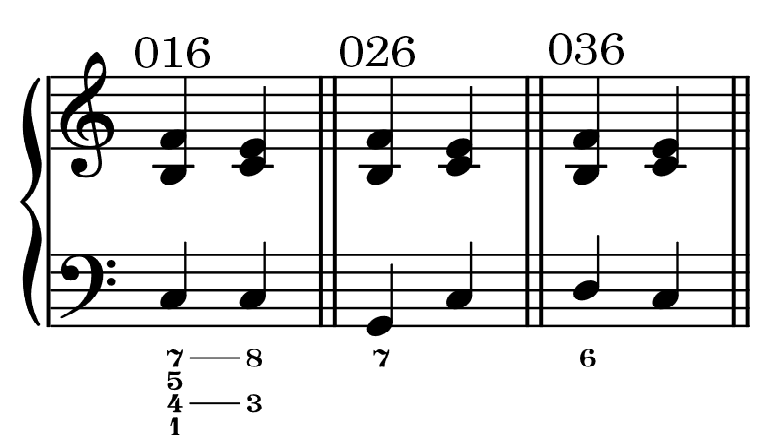
\includegraphics[width=\linewidth]{figures/cadential}%
        \caption{Diagnostic trichords of the diatonic set in cadential contexts.}
        \label{fig:cadential}
    \end{figure}

    After accounting for the information provided by both 2‑ and 3‑note combinations, we can now compare them directly.
    Although diagnostic trichords such as 016, 026, 036, 046, and 056 yield more information than any dyad, some dyads still outstrip certain trichords.
    For instance, intervals 01, 03, 04, and 06 all provide more information than the trichord 027.
    This variability highlights the need to assess entire combination spaces rather than focusing on isolated cases.

    By calculating entropy across all dyads ($\Omega_2$), we find that a random 2‑note combination provides an average of about 1.54 bits of information, leaving roughly 4.1 candidate tonics.
    For trichords ($\Omega_3$), the average rises to about 2.16 bits, leaving about 2.7 candidate tonics.
    Thus, while trichords are generally more informative, the distributions overlap enough to warrant comparison across cardinalities.

    This motivates the next step: synthesizing a value for the set as a whole.
    Such a measure reflects the average amount of information gained by any random note combination, allowing meaningful comparison between different sets.
    The method is an extension of the approach above: we compute the entropy for each cardinality and then weigh these values by their relative frequency within the set.

    Table~\ref{tab:entropy-diatonic} lists the entropy values for all cardinalities in the diatonic set, derived using binomial coefficients to enumerate the total number of combinations at each size.
    A 7‑note set yields 127 possible combinations (7+21+35+35+21+7+1).
    We therefore calculate the weighted sum of entropies as follows:

    \begin{align}
        E[I]_{\text{diatonic}} &= \sum_{k=1}^{7} \frac{\binom{7}{k}}{127} \; E_{\Omega_k}[I]
        \label{eq:diatonic-avg} \\[4pt]
        \intertext{Substituting the values from Table~\ref{tab:entropy-diatonic}:}
        E[I]_{\text{diatonic}} \;\approx\; &
        \underbrace{\left( \frac{7}{127} \cdot 0.78 \right)}_{\substack{k=1:\\ \text{weight}\cdot E_{\Omega_1}}} +
        \underbrace{\left( \frac{21}{127} \cdot 1.54 \right)}_{\substack{k=2:\\ \text{weight}\cdot E_{\Omega_2}}} +
        \underbrace{\left( \frac{35}{127} \cdot 2.16 \right)}_{\substack{k=3:\\ \text{weight}\cdot E_{\Omega_3}}}
        \notag \\[4pt]
        &+ \left( \frac{35}{127} \cdot 2.61 \right) +
        \left( \frac{21}{127} \cdot 2.98 \right)
        \notag \\[4pt]
        &+ \left( \frac{7}{127} \cdot 3.30 \right) +
        \left( \frac{1}{127} \cdot 3.58 \right)
        \;\approx\; 2.31
        \label{eq:diatonic-sub}
    \end{align}

    \begin{table}[htbp]
    \centering
    \caption{The amount of entropy in combinations of different cardinalities in the diatonic set.}
    \label{tab:entropy-diatonic}
    \begin{tabular}{c c c c}
        \toprule
            \makecell{Combination\\cardinality} &
            \makecell{Binomial\\coefficient} &
            $E[I]$ &
            \makecell{Candidate\\transpositions} \\
        \midrule
            1 & 7  & 0.78 & 7   \\
            2 & 21 & 1.54 & 4.1 \\
            3 & 35 & 2.16 & 2.7 \\
            4 & 35 & 2.61 & 2.0 \\
            5 & 21 & 2.98 & 1.5 \\
            6 & 7  & 3.30 & 1.2 \\
            7 & 1  & 3.58 & 1.0 \\
        \bottomrule
    \end{tabular}
\end{table}

    This corresponds to about $2.42$ candidate tonal interpretations on average.
    For brevity, we call this value the \emph{Tonal Ambiguity Index} (TAI) of the set:
    \[
        \mathrm{TAI}(S) \;=\; \bar{t}(S) \;=\; \frac{c}{2^{\mathbb{E}_S[I]}}.
    \]
    Smaller TAI indicates less ambiguity (fewer viable tonics); larger TAI indicates more ambiguity.

    Although the calculations rely on information theory, the intent of this framework is practical: to describe tonal ambiguity in terms accessible to musicians and theorists.
    Since raw values in bits may feel abstract, it is recommended to present ambiguity as the \textit{average number of possible tonal interpretations} (with conversion via Eq.~\ref{eq:remaining_transpositions}).
    This framing preserves mathematical rigor while ensuring interpretability in musical terms.

    \subsection{Common scales with uniqueness}

    By applying our synthesized measure of ambiguity, we can extend our understanding of scales beyond a binary classification of uniqueness.
    This measure enables direct comparison of scales in their capacity to induce tonality, both through analyses of note combinations at varying cardinalities and through set‑level evaluations.
    Table~\ref{tab:tonal-interpretations} presents ambiguity values (t) for several widely used scales, showing the number of possible tonal interpretations for note combinations ranging from one to seven notes, as well as the overall ambiguity of each set.

    On average, the major scale exhibits the greatest tonal ambiguity, with $\bar{t}\approx 2.42$ possible interpretations.
    This is followed by the pentatonic scale (t=2.29), the melodic minor (t=1.92), and the harmonic minor (t=1.87).
    Put differently, hearing a random combination of notes from the harmonic minor scale is more likely to allow its transposition to be identified unambiguously than a comparable combination drawn from the major scale.

    Importantly, these findings should not be understood merely as mathematical curiosities.
    In practical terms, they suggest that the major scale affords composers roughly 30% more opportunities to sustain tonal ambiguity than the harmonic minor.
    Thus, the measure does not simply quantify an abstract property, but also highlights a meaningful dimension of compositional practice: the degree to which a scale structurally supports or resists immediate tonal clarity.

    \begin{table}[htbp]
\setlength{\tabcolsep}{2pt} % reduce column padding
\centering
\small
\caption{Common scales and the amount of tonal ambiguity ($t$) they convey at different
combination cardinalities and within the set as a whole.}
\label{tab:tonal-interpretations}
    \begin{tabular}{l c c c c}
    \toprule
    \multicolumn{5}{c}{\textbf{Tonal Interpretations}} \\
    \midrule
    \makecell[c]{Combo\\Cardinality} &
    \makecell[c]{Major\\(024579E)} &
    \makecell[c]{Pentatonic\\(02479)} &
    \makecell[c]{Asc.\\Melodic\\Minor\\(023579E)} &
    \makecell[c]{Harmonic\\Minor\\(023578E)} \\
    \midrule
    1 & 7.00 & 5.00 & 7.00 & 7.00 \\
    2 & 4.12 & 2.78 & 3.95 & 3.89 \\
    3 & 2.69 & 1.83 & 2.21 & 2.14 \\
    4 & 1.97 & 1.32 & 1.40 & 1.32 \\
    5 & 1.52 & 1.00 & 1.07 & 1.07 \\
    6 & 1.22 & --   & 1.00 & 1.00 \\
    7 & 1.00 & --   & 1.00 & 1.00 \\
    \midrule
    \textit{Set} & 2.42 & 2.29 & 1.92 & 1.87 \\
    \bottomrule
    \end{tabular}
\end{table}

    \subsection{Modes of limited transposition}

    As noted in the introduction, modes of limited transposition were a central motivation for this study.
    Because they do not possess the uniqueness property, they present an ideal testing ground for a measure that quantifies tonal ambiguity beyond a simple binary classification.
    Their enduring popularity may well stem from precisely this balance: they convey a sense of tonality while preserving a structural ambiguity absent in unstructured atonal passages.

    Our measure of ambiguity enables a meaningful comparison among such modes, even in the absence of uniqueness.
    Table~\ref{tab:tonal-interpretations-mlt} presents three common examples: the octatonic scale (0235689E), the whole‑tone scale (02468T), and the augmented scale (03478E).
    For each, the table shows the number of tonal interpretations (t) available across different note‑combination cardinalities, as well as the overall ambiguity of the set.

    The results reveal that the whole‑tone scale is the most ambiguous, averaging t=6 possible tonal interpretations.
    The octatonic scale follows with $t \approx 4.33$, while the augmented scale exhibits the least ambiguity of the three, with $t \approx 3.49$.
    These findings underscore how, even without uniqueness, different modes of limited transposition afford markedly different capacities for sustaining tonal ambiguity.

    \begin{table}[htbp]
\setlength{\tabcolsep}{3pt} % reduce column padding for two-column layout
\centering
\caption{Tonal interpretations ($t$) available at different note-combination cardinalities in three modes of limited transposition. Grey shading indicates the values used to calculate the set-level ambiguity.}
\label{tab:tonal-interpretations-mlt}
\begin{tabular}{l c c c}
\toprule
\multicolumn{4}{c}{\textbf{Tonal Interpretations}} \\
\midrule
\makecell[c]{Combination\\Cardinality} &
\makecell[c]{Octatonic} &
\makecell[c]{Whole tone} &
\makecell[c]{Augmented} \\
\midrule
1 & 8.00 & 6.00 & 6.00 \\
2 & 5.38 & 6.00 & 3.96 \\
3 & 4.42 & 6.00 & 3.22 \\
4 & 4.08 & 6.00 & 3.00 \\
5 & 4.00 & 6.00 & 3.00 \\
6 & 4.00 & --          & 3.00 \\
7 & 4.00 & --          & --          \\
8 & 4.00 & --          & --          \\
\midrule
\textit{Set} & 4.33 & 6.00 & 3.49 \\
\bottomrule
\end{tabular}
\end{table}

    \subsection{Consolidating insights}

    Table~\ref{tab:scale-ambiguity} presents the ambiguity values for the seven common scales examined in this study.
    Crucially, this measure allows scales that possess uniqueness to be compared directly with those that do not, situating both on a single continuum of tonal ambiguity.
    Such a unified framework enables both rigorous analysis and intuitive interpretation.

    For example, we can now state not only that the octatonic scale is more ambiguous than the major scale, but quantify that it has almost twice the tonal ambiguity.
    This reframing allows us to describe and compare the tonal affordances of different
    scales in ways that are both mathematically precise and musically meaningful.

    \begin{table}[htbp]
\setlength{\tabcolsep}{4pt} % tighten column padding if needed
\centering
\caption{Popular scales and their ambiguity values. Values represent the average number of possible tonal interpretations derived from the entropy measure in Equation~\ref{eq:diatonic-avg}.}
\label{tab:scale-ambiguity}
\begin{tabular}{l c}
\toprule
\makecell[l]{Set} & \makecell[c]{Ambiguity\\Value} \\
\midrule
Harmonic Minor (023578E)         & 1.87 \\
Ascending Melodic Minor (023579E) & 1.93 \\
Major Pentatonic (02479)          & 2.29 \\
Major scale (024579E)             & 2.41 \\
Augmented (03478E)                & 3.50 \\
Octatonic (0235689E)              & 4.34 \\
Whole-tone (02468T)               & 6.00 \\
\bottomrule
\end{tabular}
\end{table}

    \paragraph{Normalization across chromatic universes.}
    For cross-EDO comparisons (chromatic size $c$), we report two dimensionless quantities:
    \[
        \mathrm{NMI}(S) \coloneqq \frac{\mathbb{E}_S[I]}{\log_2 c}
    \]
    \emph{(Normalized information; higher = less ambiguous.)}
    \[
        \mathrm{NA}(S) \coloneqq 1 - \mathrm{NMI}(S) = \frac{\log_2 \bar{t}(S)}{\log_2 c}
    \]
    \emph{(Normalized ambiguity; higher = more ambiguous.)}
    These relate to the raw ambiguity via
    \[
        \bar{t}(S) = c^{\mathrm{NA}(S)} = c^{1-\mathrm{NMI}(S)}, \qquad \mathrm{TAI}(S)=\bar{t}(S).
    \]
    In 12-EDO, $\log_2 12 \approx 3.585$, so $\mathrm{NMI}\approx \mathbb{E}_S[I]/3.585$.



    \subsection{Allowing for time}

    The ambiguity values computed thus far rest on an important assumption: that each note drawn from a scale is new, not previously heard.
    This assumption overlooks the temporal nature of music, where notes may repeat before new ones appear.
    To account for this, we can instead imagine constructing melodies by randomly drawing notes from a scale and then tallying the number of \textit{distinct} pitches in the result.
    Rather than averaging across all possible combinations in every cardinality, this approach focuses on the combinations most likely to occur, yielding a more nuanced and musically representative measure of ambiguity.

    To illustrate, consider constructing an eight‑note melody from the C major scale, such as A–C–G–G–E–C–A–E.
This melody consists of four distinct pitches: A, C, G, and E.
    Using the methods outlined previously, we can compute the self‑information provided by this specific subset.
    Hearing these notes reduces the space of possible transpositions from 12 to just three tonal interpretations: C major, F major, and G major.
    Of course, there is no guarantee that a random draw of eight notes would yield these particular four.
    Another melody of the same length might contain as many as seven distinct notes (C–D–E–F–G–A–B) or as few as one (e.g., D repeated).
    Thus, to calculate the expected information from an eight‑note melody, we must first determine the average number of distinct notes we are likely to encounter.

    This requires introducing a new weighting scheme for the number of distinct pitches produced, enabling us to compute a weighted average across multiple cardinalities.
    Specifically, we must determine the probability $P_k$ of ending up with a melody containing exactly $k$ distinct pitches.
    These probabilities can then be used as weights for the $\mathbb{E}[I]$ values corresponding to each cardinality (as specified in Table~\ref{tab:entropy-diatonic}).

    The probability of drawing exactly $k$ distinct pitches when selecting $n$ notes from a scale of cardinality $m$ is given by \citet{Feller1968}:

    \begin{equation}
        P_k = m^{-n} \, \left\langle \genfrac{}{}{0pt}{}{n}{k} \right\rangle \binom{m}{k} \, k!
        \label{eq:Pk}
    \end{equation}

    For example, drawing $n = 8$ notes from the diatonic scale ($m = 7$) produces:

    \begin{align*}
        P_1 = 7^{-8} \, \Stirling{8}{1} \, \binom{7}{1} \cdot 1! \\
        &= 7^{-8} \cdot 1 \cdot 7 \cdot 1
        \approx 0.000
    \end{align*}

    For two distinct notes:

    \begin{align*}
        P_2 = 7^{-8} \, \Stirling{8}{2} \, \binom{7}{2} \cdot 2! \\
        &= 7^{-8} \cdot 127 \cdot 21 \cdot 2
        \approx 0.001
    \end{align*}

    And so on:
    \begin{align*}
        P_3 &\approx 0.035, \quad
        P_4 \approx 0.248, \quad
        P_5 \approx 0.459, \\
        P_6 &\approx 0.233, \quad
        P_7 \approx 0.024.
    \end{align*}

    Applying these probabilities as weights to the corresponding entropy values yields:
    \[
        P_1 \cdot E_{\text{set}~\Omega_1}[I] \;+\; \cdots \;+\; P_7 \cdot E_{\text{set}~\Omega_7}[I]
        \;\approx\; 2.95 \ \text{bits}.
    \]

    This result indicates that, on average, eight random draws from the diatonic scale reduce the transpositional space from 12 to about 1.55 candidate tonal interpretations.

    \autoref{fig:wide} shows how the amount of information gained varies with melody length across several common scales.
    The octatonic scale begins with eight candidate tonalities and converges to four.
    The whole‑tone scale remains fixed at six throughout.
    The major, harmonic minor, and ascending melodic minor each begin with seven and converge rapidly to uniqueness (one interpretation).
    The pentatonic scale begins with five and eventually converges to uniqueness as well, though somewhat more slowly than the minor scales

    \begin{figure*}[htbp]
        \centering
        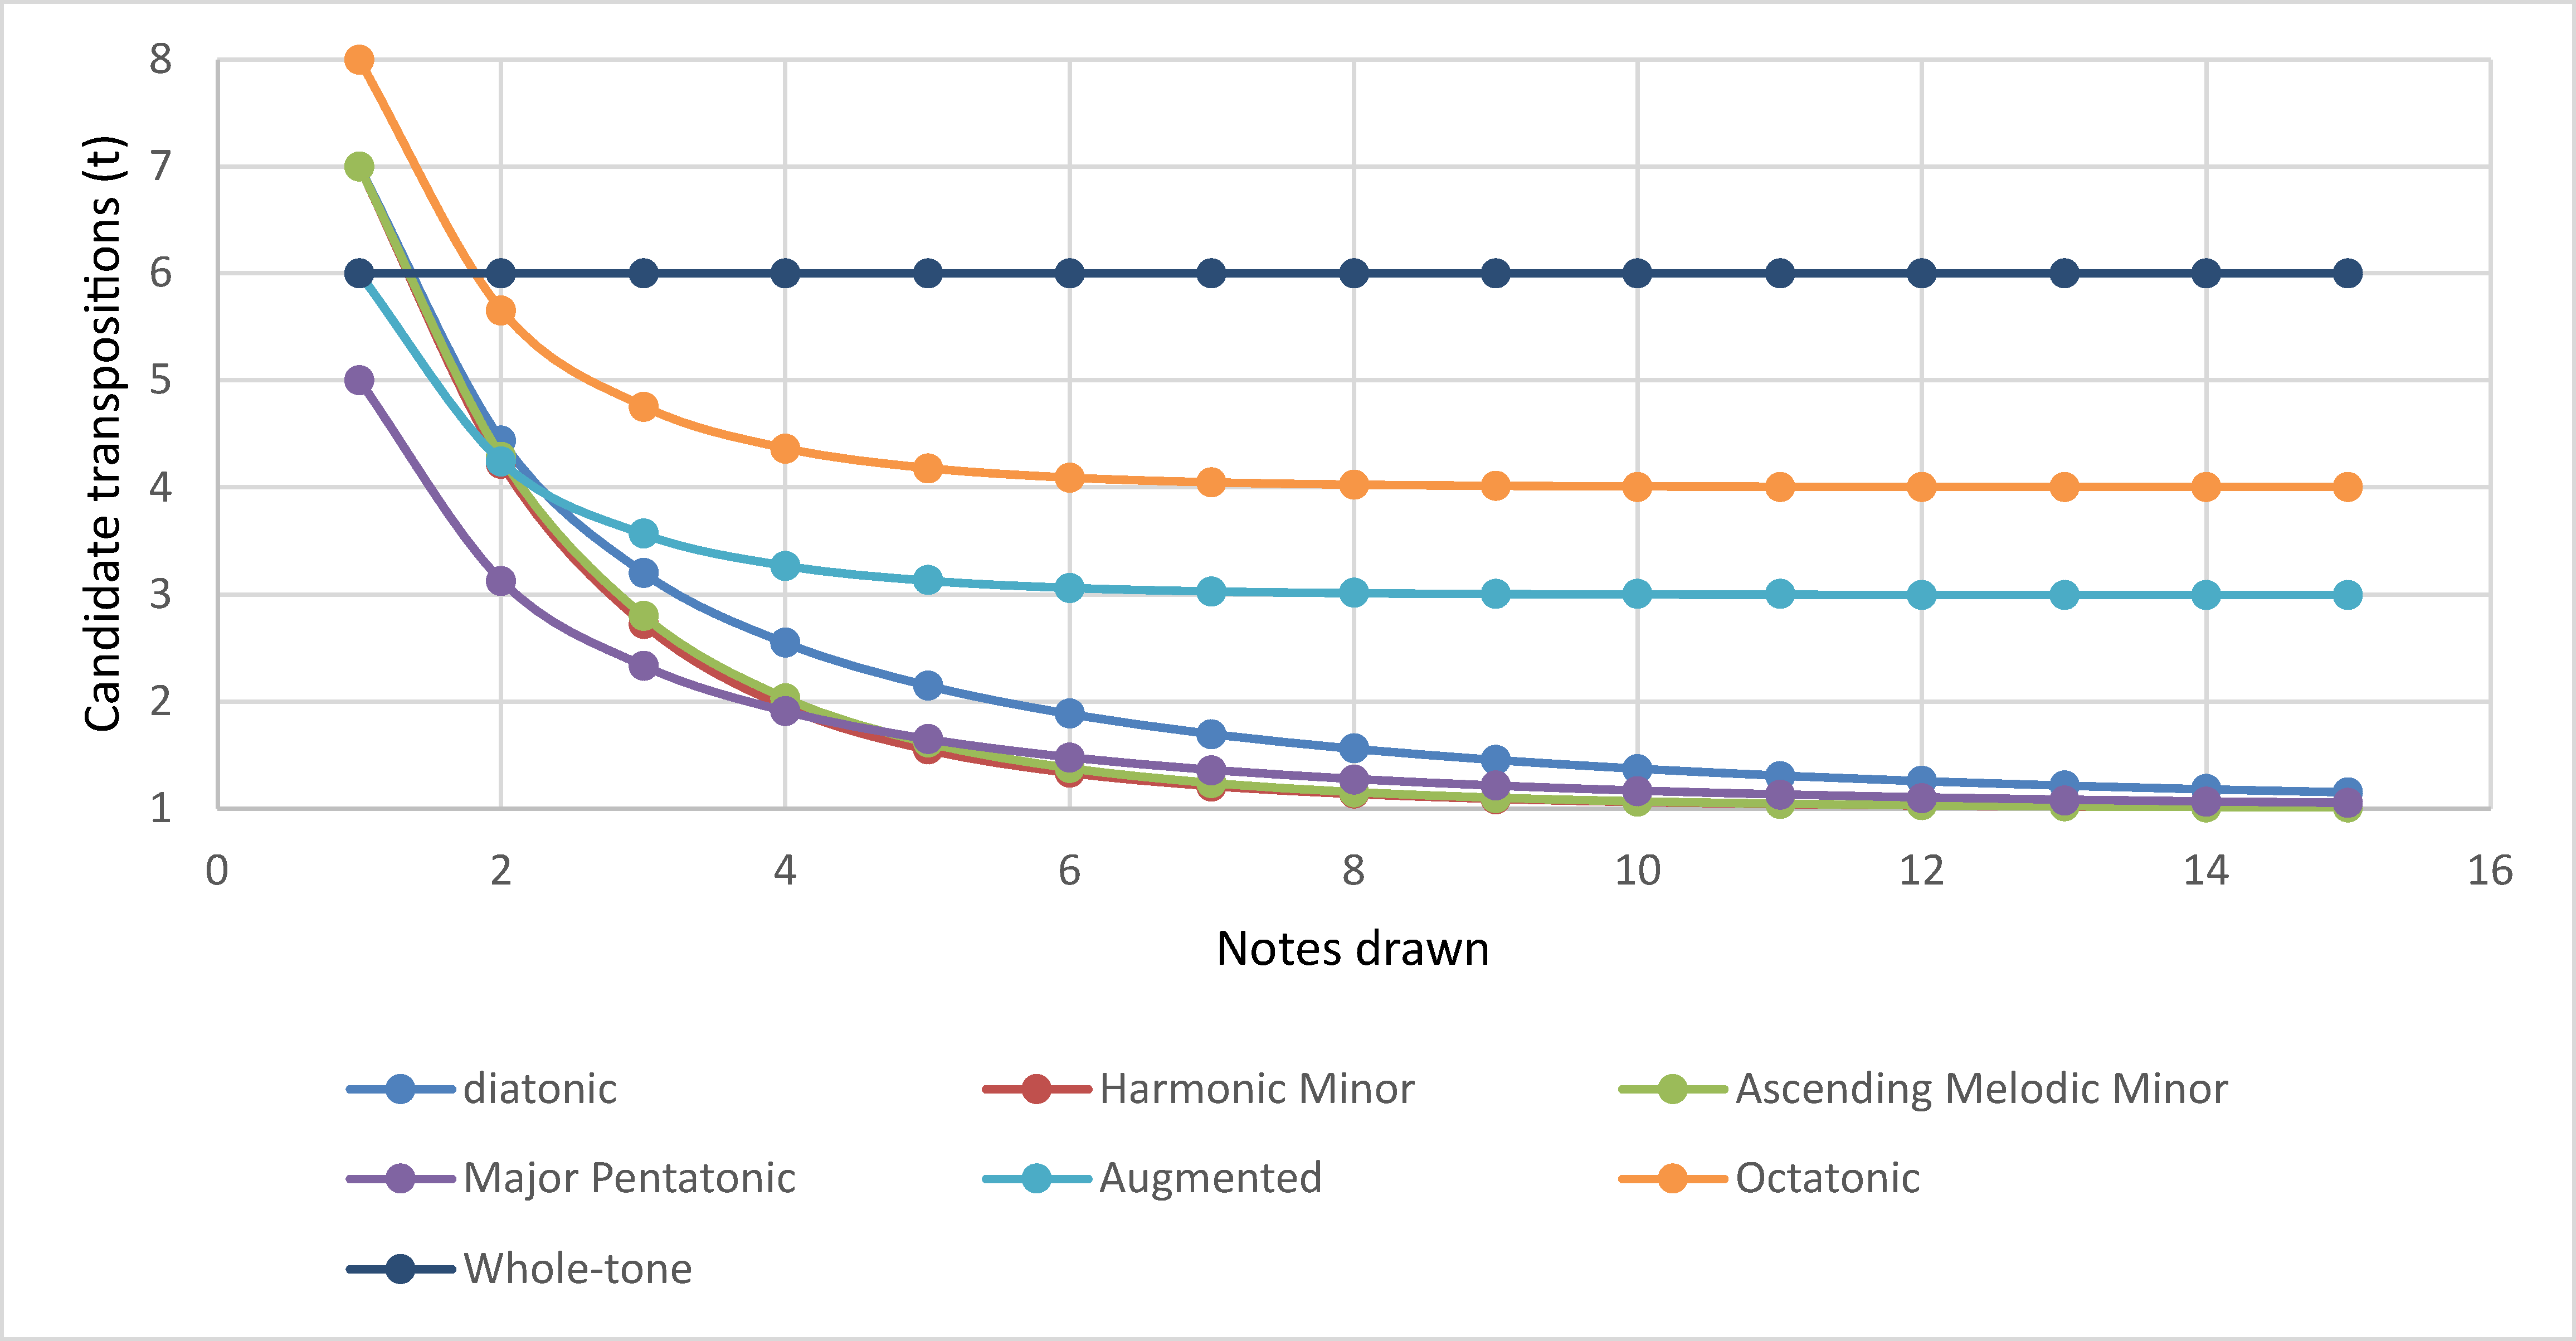
\includegraphics[width=0.9\textwidth]{transposition-probability.pdf}%
        \caption{The number of tonal interpretations available in common scales as a function of the number of notes drawn from them at random.
        The y‑axis represents the number of tonal interpretations available.
        The x‑axis refers to the number of draws.
        These values were computed using Eq.~\ref{eq:Pk}.}
        \label{fig:wide}
    \end{figure*}

    But how do we determine the appropriate number of notes to draw to represent a set?
    As \autoref{fig:time} illustrates, the extremes each present problems.
    A single note offers virtually no information about the set, while an infinite sequence of notes drives the measure toward the minimal ambiguity value, obscuring the subtler tonal distinctions.
    For practical purposes, eight notes were chosen as a compromise: enough to allow full representation even in eight‑note sets such as the octatonic, yet not so many as to guarantee convergence.
    Still, this remains an arbitrary decision.

    \begin{figure*}[htbp]
        \centering
        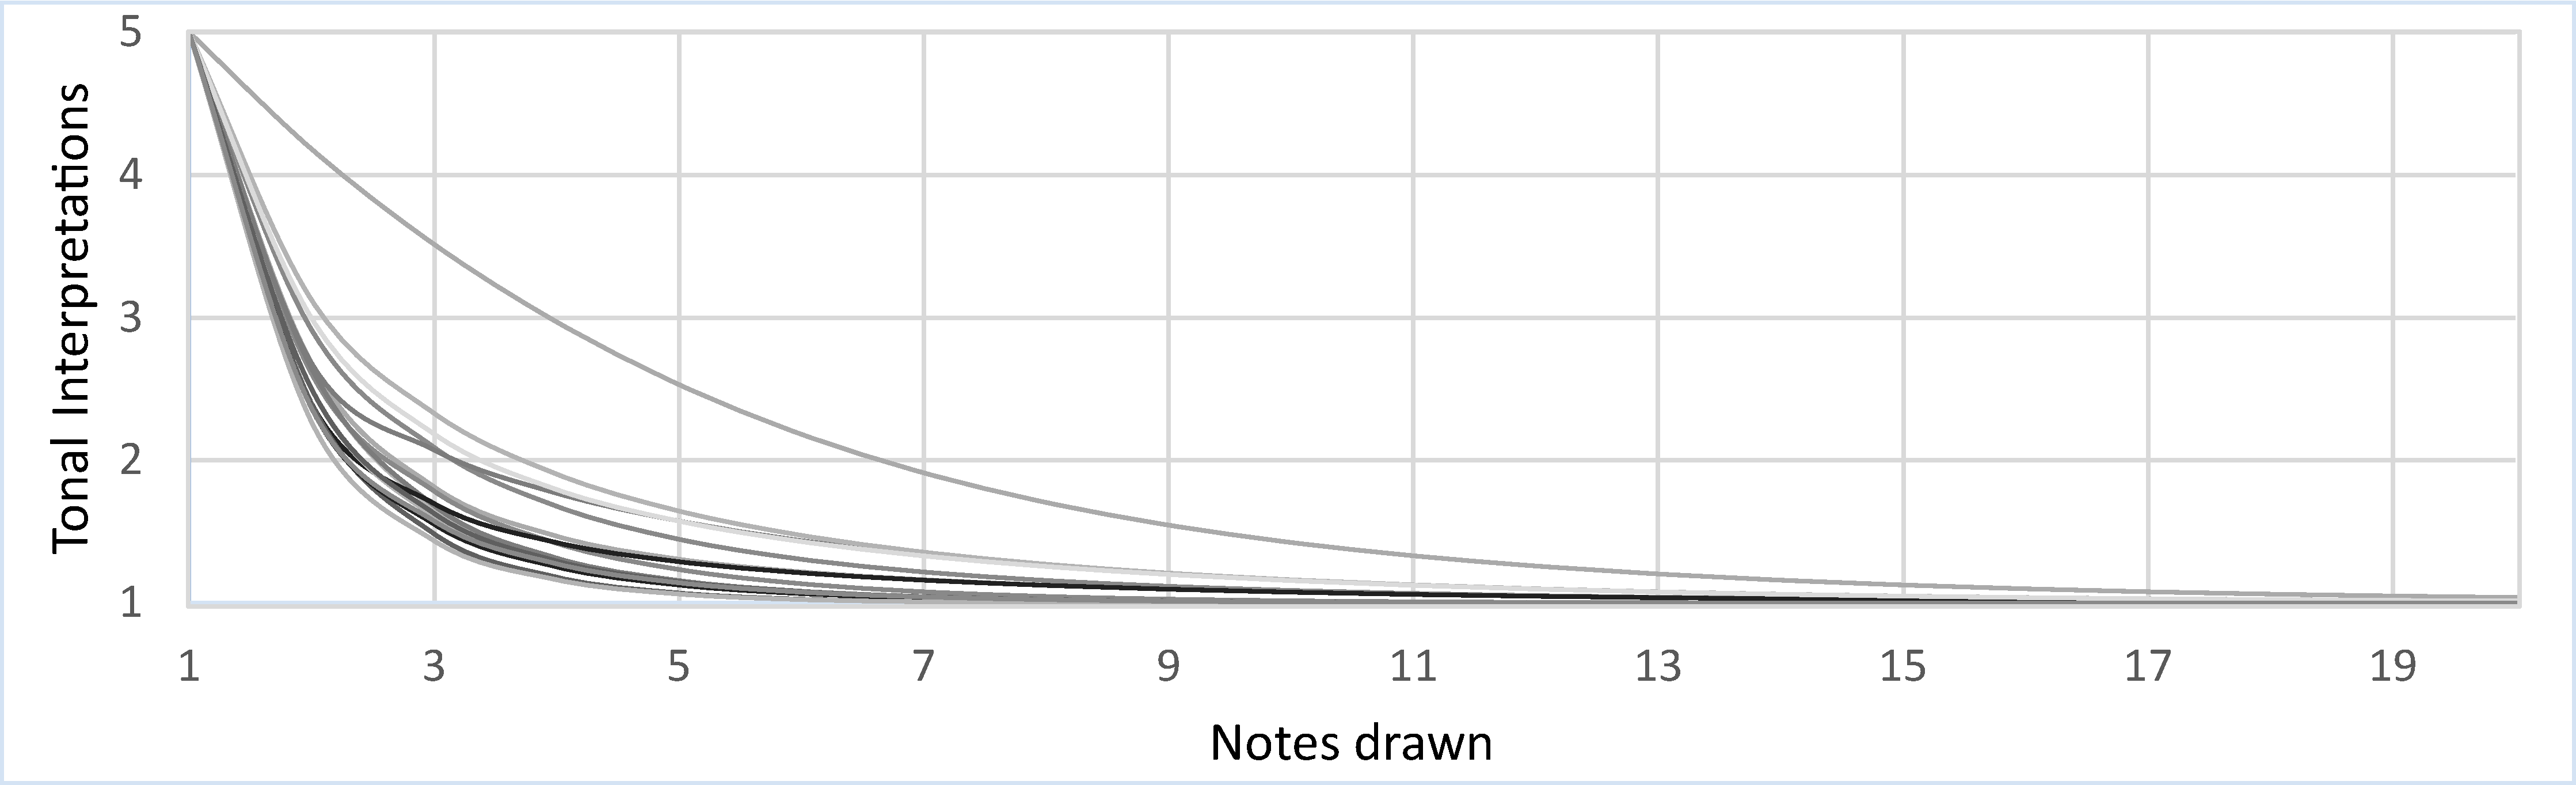
\includegraphics[width=0.9\textwidth]{transposition-time.pdf}%
        \caption{All 5‑note sets in 12-EDO (twelve equal divisions of the octave) and the number of tonal interpretations they leave as a function of the number of notes drawn at random from the set.}
        \label{fig:time}
    \end{figure*}

    One possible method of summarizing the temporal behavior of a set is to measure the \textit{area under the convergence curve} (AUC).
    In this framing, the slower a scale converges, the larger the enclosed area.
    However, this approach has three notable drawbacks.
    First, computing AUC is more complex than earlier calculations.
    Second, the AUC reflects only the \textit{rate} of convergence, not the \textit{extent} of ambiguity.
    For example, the octatonic scale converges quickly to three interpretations ($AUC \approx 0.946$), while the major scale converges more slowly ($AUC \approx 3.803$).
    Third—and most importantly—AUC values are difficult to interpret musically.

    That said, AUC and ambiguity values are highly correlated ($r^2 > 0.98$ for both 5‑ and 7‑note scales), suggesting a strong intrinsic relationship.
    Thus, while AUC may serve as a form of validation, the ambiguity values developed earlier remain preferable: they are rigorous, musically interpretable, and provide a direct means of quantifying tonal ambiguity across different sets.

    \subsection{Disambiguating Sets}

    Up to this point, our formalization of tonal ambiguity has assumed that the underlying set was known.
    In other words, we worked within the framework of a given scale and sought to determine the transposition in which it manifested, based on combinations of different cardinalities.
    Yet in real listening contexts, this assumption is not always justified.
    While certain scale structures are often present as a priori expectations\citep{Krumhansl1979}, listeners must also identify not only the tonic but the very set or mode that scaffolds a passage.
    Thus, the task is not merely to decide that a piece is in C, but whether it is in C major, C minor, or another set entirely.

    To address this, we can shift focus from measuring a set's ambiguity internally to examining a note‑combination's ability to \textit{disambiguate between different sets}.
    For example, if we hear the combination 014, can we determine which set is in use, or at least eliminate certain sets as possibilities?
    Formally, the answer is "barely," but in practice—since not all sets occur with equal frequency—the answer may well be "yes."

    Table~\ref{tab:comb-cardinality} presents the average number of possible seven‑note sets remaining after eliminating candidates based on note combinations of varying cardinalities.
    Across the 66 distinct 7‑note sets in 12‑EDO, the results appear daunting: even after hearing five of the seven notes, an average of nearly 20 candidate sets remain.
    The most diagnostic combination, 01369, still leaves 13 possibilities.
    Identifying a specific set among the full field of 66 thus seems highly impractical.

    \begin{table}[htbp]
\setlength{\tabcolsep}{4pt} % adjust column padding for tight layouts
\centering
\caption{Note combinations of different cardinalities and their ability to identify specific 7-note sets.}
\label{tab:comb-cardinality}
\begin{tabular}{c c}
\toprule
\makecell[c]{Combination\\cardinality} &
\makecell[c]{Possible sets\\on average (range)} \\
\midrule
1 & 66 (66) \\
2 & 66 (66) \\
3 & 62.8 (39--65) \\
4 & 43 (14--48) \\
5 & 19.3 (13--21) \\
6 & 5.7 (1--6) \\
\bottomrule
\end{tabular}
\end{table}

    However, as previously noted, not all sets are equally likely in Western music.
    In fact, the effective pool of candidates is much smaller, consisting primarily of the diatonic set (major and its modes), the harmonic and melodic minors, the major pentatonic and its modes, the whole‑tone scale, and the octatonic scale.
    The precise list may vary slightly, but the principle remains: real‑world listening involves a limited set of common tonal frameworks.

    Within this restricted pool, identifying the scaffolding set becomes far more practical.
    Table~\ref{tab:avg-viable-sets} displays the average number of viable candidates remaining when restricting analysis to these six common scales.
    The results suggest that certain combinations may serve as useful heuristics in real‑world listening.
    For example, the presence of 0145 virtually guarantees the harmonic minor, while 0167 is most likely to be heard in the context of the octatonic scale.

    \begin{table}[htbp]
\setlength{\tabcolsep}{4pt} % tighten column padding if needed
\centering
\caption{Average number of remaining viable common sets given combinations of different cardinalities.}
\label{tab:avg-viable-sets}
\begin{tabular}{c c}
\toprule
\makecell[c]{Combination\\cardinality} &
\makecell[c]{Possible sets\\on average (range)} \\
\midrule
1 & 6 \\
2 & 5.2 (4--6) \\
3 & 4.1 (3--5) \\
4 & 2.9 (1--4) \\
5 & 1.9 (1--4) \\
6 & 1.3 (1--2) \\
\bottomrule
\end{tabular}
\end{table}

    \subsection{Conclusion}

    The property of uniqueness provides complete orientation within a collection of notes, ensuring that its transposition can be identified without ambiguity.
    In scales that fulfill uniqueness, this property supports the emergence of a clear and singular tonality.
    Yet if we allow that tonality can tolerate some degree of uncertainty, uniqueness alone proves too restrictive a condition for the presence of hierarchical relationships among a scale's notes.
    As such, uniqueness cannot capture the gradient nature of tonal clarity across different note collections.

    This paper has therefore proposed an additional measure: a quantification of the extent of tonal ambiguity within any given collection of notes.
    Unlike uniqueness, which is binary, this measure places both unique and non‑unique scales on a single continuum, offering a more nuanced view of how well a set can support tonal organization.

    The measure was formalized through methods drawn from information theory, relying on established mathematical tools for quantifying information.
    Using this framework, we examined the information gained from note combinations of varying cardinalities, explored entropy as a means of averaging across these combinations, and considered the temporal dimension by modeling melodies as sequences of notes rather than static sets.
    We also addressed the limitations of subset analysis in disambiguating between different sets.
    While in theory many sets remain possible candidates after hearing even several notes, in practice the restricted pool of commonly used scales in Western music makes disambiguation more feasible.
    Measuring a note combination's ability to exclude certain sets, rather than identify one uniquely, thus provides a more practical understanding of tonal induction.

    An appendix to this paper lists every combination of one to six notes in 12‑EDO, showing both the number of tonal interpretations that remain in the context of the scales discussed and the number of viable candidate sets.
    This comprehensive resource supports further application of the ambiguity measure and demonstrates its utility for music theory and analysis.

% --- References (natbib) ---
    \bibliographystyle{apalike}
    \bibliography{refs}

    \clearpage

% Shading helpers
    \newcommand{\sone}[1]{\cellcolor{gray!20}{#1}} % single interpretation "1"
    \newcommand{\diag}{\rowcolor{green!12}}        % Possible Sets = 1 row highlight

% ---------- Appendix: full table ----------
    \section*{Appendix: Possible Transpositions by Combination}

    % ---- begin squeeze ----
    \begingroup
    \footnotesize                           % smaller font (try \footnotesize if this is too small)
%    \setlength{\tabcolsep}{2.2pt}         % narrower column padding (default is 6pt)
%    \renewcommand{\arraystretch}{0.9}     % tighter rows (1.0 is default)

% (optional) slightly tighter booktabs spacing
    \setlength{\aboverulesep}{0.3ex}
    \setlength{\belowrulesep}{0.3ex}

% Repeated head/foot for supertabular
    \tablefirsthead{%
        \toprule
        \makecell[l]{Combo} &
        \makecell[c]{M} & \makecell[c]{mm} & \makecell[c]{hm} &
        \makecell[c]{WT} & \makecell[c]{O} & \makecell[c]{P} &
        \makecell[c]{A} & \makecell[c]{Possible\\Sets} \\
        \midrule
    }
    \tablehead{%
        \toprule
        \makecell[l]{Combo} &
        \makecell[c]{M} & \makecell[c]{mm} & \makecell[c]{hm} &
        \makecell[c]{WT} & \makecell[c]{O} & \makecell[c]{P} &
        \makecell[c]{A} & \makecell[c]{Possible\\Sets} \\
        \midrule
    }
    \tabletail{%
        \midrule
        \multicolumn{9}{r}{\emph{Continued on next column/page}}\\
    }
    \tablelasttail{\bottomrule}

% your table content:
    \begin{center}
\tablecaption{Every note combination with 1–6 notes in 12 EDO, showing the number of possible transpositions within seven common scales and the number of possible sets (M = Major, mm = Asc.\ Melodic Minor, hm = Harmonic Minor, WT = Whole-Tone, O = Octatonic, P = Major Pentatonic, A = Augmented). Gray cells mark single interpretations (1); light-green rows mark combinations whose \emph{Possible Sets} equals 1.}
\label{tab:appendix-transpositions}
\begin{supertabular}{l c c c c c c c c}
% ---- FULL DATA (transcribed) ----
% ---- length 1 (single digit) ----
0    & 7 & 7 & 7 & \sone{1} & 2 & 5 & 6 & 7 \\

% ---- length 2 (two digits) ----
01   & 2 & 2 & 3 & -- & \sone{1} & -- & 3 & 5 \\
02   & 5 & 5 & 3 & \sone{1} & \sone{1} & 3 & -- & 6 \\
03   & 4 & 4 & 5 & -- & 2 & 2 & 3 & 6 \\
04   & 3 & 4 & 4 & \sone{1} & \sone{1} & \sone{1} & 6 & 7 \\
05   & 6 & 4 & 4 & -- & \sone{1} & 4 & 3 & 6 \\
06   & 2 & 4 & 4 & \sone{1} & 2 & -- & -- & 5 \\

% ---- length 3 ----
013  & 2 & 2 & 2 & -- & \sone{1} & -- & -- & 4 \\
014  & -- & \sone{1} & 2 & -- & \sone{1} & -- & 3 & 4 \\
015  & 2 & \sone{1} & 2 & -- & -- & -- & 3 & 4 \\
016  & \sone{1} & \sone{1} & 2 & -- & \sone{1} & -- & -- & 4 \\
023  & 2 & 2 & 2 & -- & \sone{1} & -- & -- & 4 \\
024  & 3 & 3 & \sone{1} & \sone{1} & -- & \sone{1} & -- & 5 \\
025  & 4 & 3 & 2 & -- & \sone{1} & 2 & -- & 5 \\
026  & \sone{1} & 3 & \sone{1} & \sone{1} & \sone{1} & -- & -- & 5 \\
027  & 5 & 3 & 2 & -- & -- & 3 & -- & 4 \\
034  & -- & \sone{1} & 2 & -- & \sone{1} & -- & 3 & 4 \\
035  & 4 & 3 & 2 & -- & \sone{1} & 2 & -- & 5 \\
036  & \sone{1} & 2 & 4 & -- & 2 & -- & -- & 4 \\
037  & 3 & 2 & 3 & -- & \sone{1} & \sone{1} & 3 & 6 \\
045  & 2 & \sone{1} & 2 & -- & -- & -- & 3 & 4 \\
046  & \sone{1} & 3 & 2 & \sone{1} & \sone{1} & -- & -- & 5 \\
047  & 3 & 2 & 2 & -- & \sone{1} & \sone{1} & 3 & 6 \\
048  & -- & 3 & 3 & \sone{1} & -- & -- & 6 & 4 \\
056  & \sone{1} & \sone{1} & \sone{1} & -- & \sone{1} & -- & -- & 4 \\

% ---- length 4 ----
0134 & -- & \sone{1} & \sone{1} & -- & \sone{1} & -- & -- & 3 \\
0135 & 2 & \sone{1} & \sone{1} & -- & -- & -- & -- & 3 \\
0136 & \sone{1} & \sone{1} & 2 & -- & \sone{1} & -- & -- & 4 \\
0137 & \sone{1} & \sone{1} & -- & -- & \sone{1} & -- & -- & 3 \\
0145 & -- & -- & \sone{1} & -- & -- & -- & 3 & 2 \\
0146 & -- & \sone{1} & \sone{1} & -- & \sone{1} & -- & -- & 3 \\
0147 & -- & -- & \sone{1} & -- & \sone{1} & -- & -- & 2 \\
0148 & -- & \sone{1} & 2 & -- & -- & -- & 3 & 3 \\
0156 & \sone{1} & -- & \sone{1} & -- & -- & -- & -- & 2 \\
0157 & \sone{1} & \sone{1} & \sone{1} & -- & -- & -- & -- & 3 \\
0158 & 2 & -- & \sone{1} & -- & -- & -- & 3 & 3 \\
0235 & 2 & 2 & \sone{1} & -- & \sone{1} & -- & -- & 4 \\
0236 & -- & \sone{1} & \sone{1} & -- & \sone{1} & -- & -- & 3 \\
0237 & 2 & \sone{1} & 2 & -- & -- & -- & -- & 3 \\
0245 & 2 & \sone{1} & \sone{1} & -- & -- & -- & -- & 3 \\
0246 & \sone{1} & 2 & -- & \sone{1} & -- & -- & -- & 3 \\
0247 & 3 & 2 & -- & -- & -- & \sone{1} & -- & 3 \\
0248 & -- & 2 & \sone{1} & \sone{1} & -- & -- & -- & 3 \\
0256 & -- & \sone{1} & -- & -- & \sone{1} & -- & -- & 2 \\
0257 & 4 & 2 & \sone{1} & -- & -- & 2 & -- & 4 \\
0258 & \sone{1} & 2 & 2 & -- & \sone{1} & -- & -- & 4 \\
0267 & \sone{1} & \sone{1} & \sone{1} & -- & -- & -- & -- & 3 \\
0268 & -- & 2 & -- & \sone{1} & \sone{1} & -- & -- & 3 \\
0346 & -- & \sone{1} & 2 & -- & \sone{1} & -- & -- & 3 \\
0347 & -- & -- & \sone{1} & -- & \sone{1} & -- & 3 & 3 \\
0348 & -- & \sone{1} & \sone{1} & -- & -- & -- & 3 & 3 \\
0356 & \sone{1} & \sone{1} & \sone{1} & -- & \sone{1} & -- & -- & 4 \\
0357 & 3 & 2 & \sone{1} & -- & -- & \sone{1} & -- & 4 \\
0358 & 3 & \sone{1} & \sone{1} & -- & \sone{1} & \sone{1} & -- & 5 \\
0367 & -- & -- & 2 & -- & \sone{1} & -- & -- & 2 \\
0368 & \sone{1} & 2 & \sone{1} & -- & \sone{1} & -- & -- & 4 \\
0369 & -- & -- & 4 & -- & \sone{1} & -- & -- & 2 \\
0467 & \sone{1} & \sone{1} & \sone{1} & -- & \sone{1} & -- & -- & 4 \\

% ---- length 5 ----
01346 & -- & \sone{1} & \sone{1} & -- & \sone{1} & -- & -- & 3 \\
\diag 01457 & -- & -- & \sone{1} & -- & -- & -- & -- & 1 \\
01458 & -- & -- & \sone{1} & -- & -- & -- & 3 & 2 \\
\diag 01467 & -- & -- & -- & -- & \sone{1} & -- & -- & 1 \\
01468 & -- & \sone{1} & \sone{1} & -- & -- & -- & -- & 2 \\
01469 & -- & -- & \sone{1} & -- & \sone{1} & -- & -- & 2 \\
\diag 01478 & -- & -- & \sone{1} & -- & -- & -- & -- & 1 \\
\diag 014589 & -- & -- & -- & -- & -- & -- & 3 & 1 \\
01568 & \sone{1} & -- & -- & -- & -- & -- & -- & 1 \\
02356 & -- & \sone{1} & -- & -- & 4 & -- & -- & 2 \\
02357 & 2 & \sone{1} & \sone{1} & -- & -- & -- & -- & 3 \\
02358 & \sone{1} & \sone{1} & \sone{1} & -- & \sone{1} & -- & -- & 4 \\
\diag 02367 & -- & -- & \sone{1} & -- & -- & -- & -- & 1 \\
02368 & -- & \sone{1} & -- & -- & \sone{1} & -- & -- & 2 \\
02369 & -- & -- & \sone{1} & -- & \sone{1} & -- & -- & 2 \\
02378 & \sone{1} & -- & \sone{1} & -- & -- & -- & -- & 2 \\
02457 & 2 & \sone{1} & -- & -- & -- & -- & -- & 2 \\
02458 & -- & \sone{1} & \sone{1} & -- & -- & -- & -- & 2 \\
02467 & \sone{1} & \sone{1} & -- & -- & -- & -- & -- & 2 \\
02468 & -- & \sone{1} & -- & \sone{1} & -- & -- & -- & 2 \\
02469 & \sone{1} & 2 & -- & -- & -- & -- & -- & 2 \\
\diag 02478 & -- & \sone{1} & -- & -- & -- & -- & -- & 1 \\
02479 & 3 & \sone{1} & -- & -- & -- & \sone{1} & -- & 3 \\
02568 & -- & \sone{1} & -- & -- & \sone{1} & -- & -- & 2 \\
\diag 02569 & -- & -- & -- & -- & \sone{1} & -- & -- & 1 \\
02578 & \sone{1} & \sone{1} & \sone{1} & -- & -- & -- & -- & 3 \\
03467 & -- & -- & \sone{1} & -- & 4 & -- & -- & 2 \\
03468 & -- & \sone{1} & \sone{1} & -- & -- & -- & -- & 2 \\
\diag 03478 & -- & -- & -- & -- & -- & -- & 3 & 1 \\
03568 & \sone{1} & \sone{1} & -- & -- & \sone{1} & -- & -- & 3 \\
03578 & 2 & -- & \sone{1} & -- & -- & -- & -- & 2 \\

% ---- length 6 (and T) ----
\diag 013467 & -- & -- & -- & -- & \sone{1} & -- & -- & 1 \\
013468 & -- & \sone{1} & \sone{1} & -- & -- & -- & -- & 2 \\
013469 & -- & -- & \sone{1} & -- & \sone{1} & -- & -- & 2 \\
\diag 013479 & -- & -- & -- & -- & \sone{1} & -- & -- & 1 \\
\diag 013568 & \sone{1} & -- & -- & -- & -- & -- & -- & 1 \\
\diag 013569 & -- & -- & \sone{1} & -- & -- & -- & -- & 1 \\
\diag 013578 & \sone{1} & -- & -- & -- & -- & -- & -- & 1 \\
\diag 013579 & -- & \sone{1} & -- & -- & -- & -- & -- & 1 \\
\diag 013679 & -- & -- & -- & -- & \sone{1} & -- & -- & 1 \\
\diag 014578 & -- & -- & \sone{1} & -- & -- & -- & -- & 1 \\
023568 & -- & \sone{1} & -- & -- & \sone{1} & -- & -- & 2 \\
\diag 023569 & -- & -- & -- & -- & \sone{1} & -- & -- & 1 \\
023578 & \sone{1} & -- & \sone{1} & -- & -- & -- & -- & 2 \\
023579 & \sone{1} & \sone{1} & -- & -- & -- & -- & -- & 2 \\
\diag 023679 & -- & -- & \sone{1} & -- & -- & -- & -- & 1 \\
\diag 024578 & -- & \sone{1} & -- & -- & -- & -- & -- & 1 \\
\diag 024589 & -- & -- & \sone{1} & -- & -- & -- & -- & 1 \\
024679 & \sone{1} & \sone{1} & -- & -- & -- & -- & -- & 2 \\
\diag 024689 & -- & \sone{1} & -- & -- & -- & -- & -- & 1 \\
\diag 02468T & -- & -- & -- & \sone{1} & -- & -- & -- & 1 \\
\diag 024579 & 2 & -- & -- & -- & -- & -- & -- & 1 \\
\diag 014679 & -- & -- & -- & -- & \sone{1} & -- & -- & 1 \\

% ---- end full list ----
\end{supertabular}
\end{center}


    \endgroup
% ---- end squeeze ----

    \paragraph{How to reproduce values in appendix}
    \small
    For each set $S\subset\mathbb{Z}_c$ and cardinality $k$:
    (1) enumerate all $k$-subsets $X\subseteq S$ (or group by isomorphism for dyads via the interval vector);
    (2) compute $t_S(X)=|\{\tau : X\subseteq\tau{+}S\}|$;
    (3) set $I_S(X)=\log_2(c/t_S(X))$ and average over $X$ to obtain $\mathbb{E}_{\Omega_k(S)}[I]$;
    (4) aggregate across cardinalities with weights $\binom{|S|}{k}/(2^{|S|}-1)$ to get $\mathbb{E}_S[I]$ and report $\mathrm{TAI}(S)=c/2^{\mathbb{E}_S[I]}$.
    For time‑aware results at length $n$, weight the cardinality‑specific expectations by $P_k$ from Eq.~\ref{eq:Pk}.



\end{document}